\section{Caching}

\begin{frame}{Intro}

	Solution: Caching\\
	\spc
	Caching is:
	\begin{itemize}
		\item We have a slow medium
		\item Add a fast medium in a data path
		\item Transparently store the data that are intended for the 
			slower medium.
		\item Profit: later accesses to the same data are faster
	\end{itemize}
	\dspc
	Sounds familiar?

	\note[item]{Η κλασσική λύση σε τέτοια προβλήματα είναι η χρήση ενός 
		γρηγορότερου αποθηκευτικού μέσου για caching.}
	\note[item]{Για όσους δεν ξέρουν τι σημαίνει caching, θα το εξηγήσουμε 
		συνοπτικά: έχεις ροή δεδομένων, καταλήγουν σε αργό μέσο, βάζεις μπροστά 
		ένα μικρό αλλά γρήγορο μέσο, οι επόμενες προσβάσεις στη μνήμη θα είναι 
		πιο γρήγορες}
	\note[item]{Γιατί δε βάζεις μόνο γρήγορο, γιατί είναι ακριβά}
	\note[item]{Προφανώς αυτό το concept είναι γνωστό. Από που;}
\end{frame}

\begin{frame}
	\makebox[\textwidth]{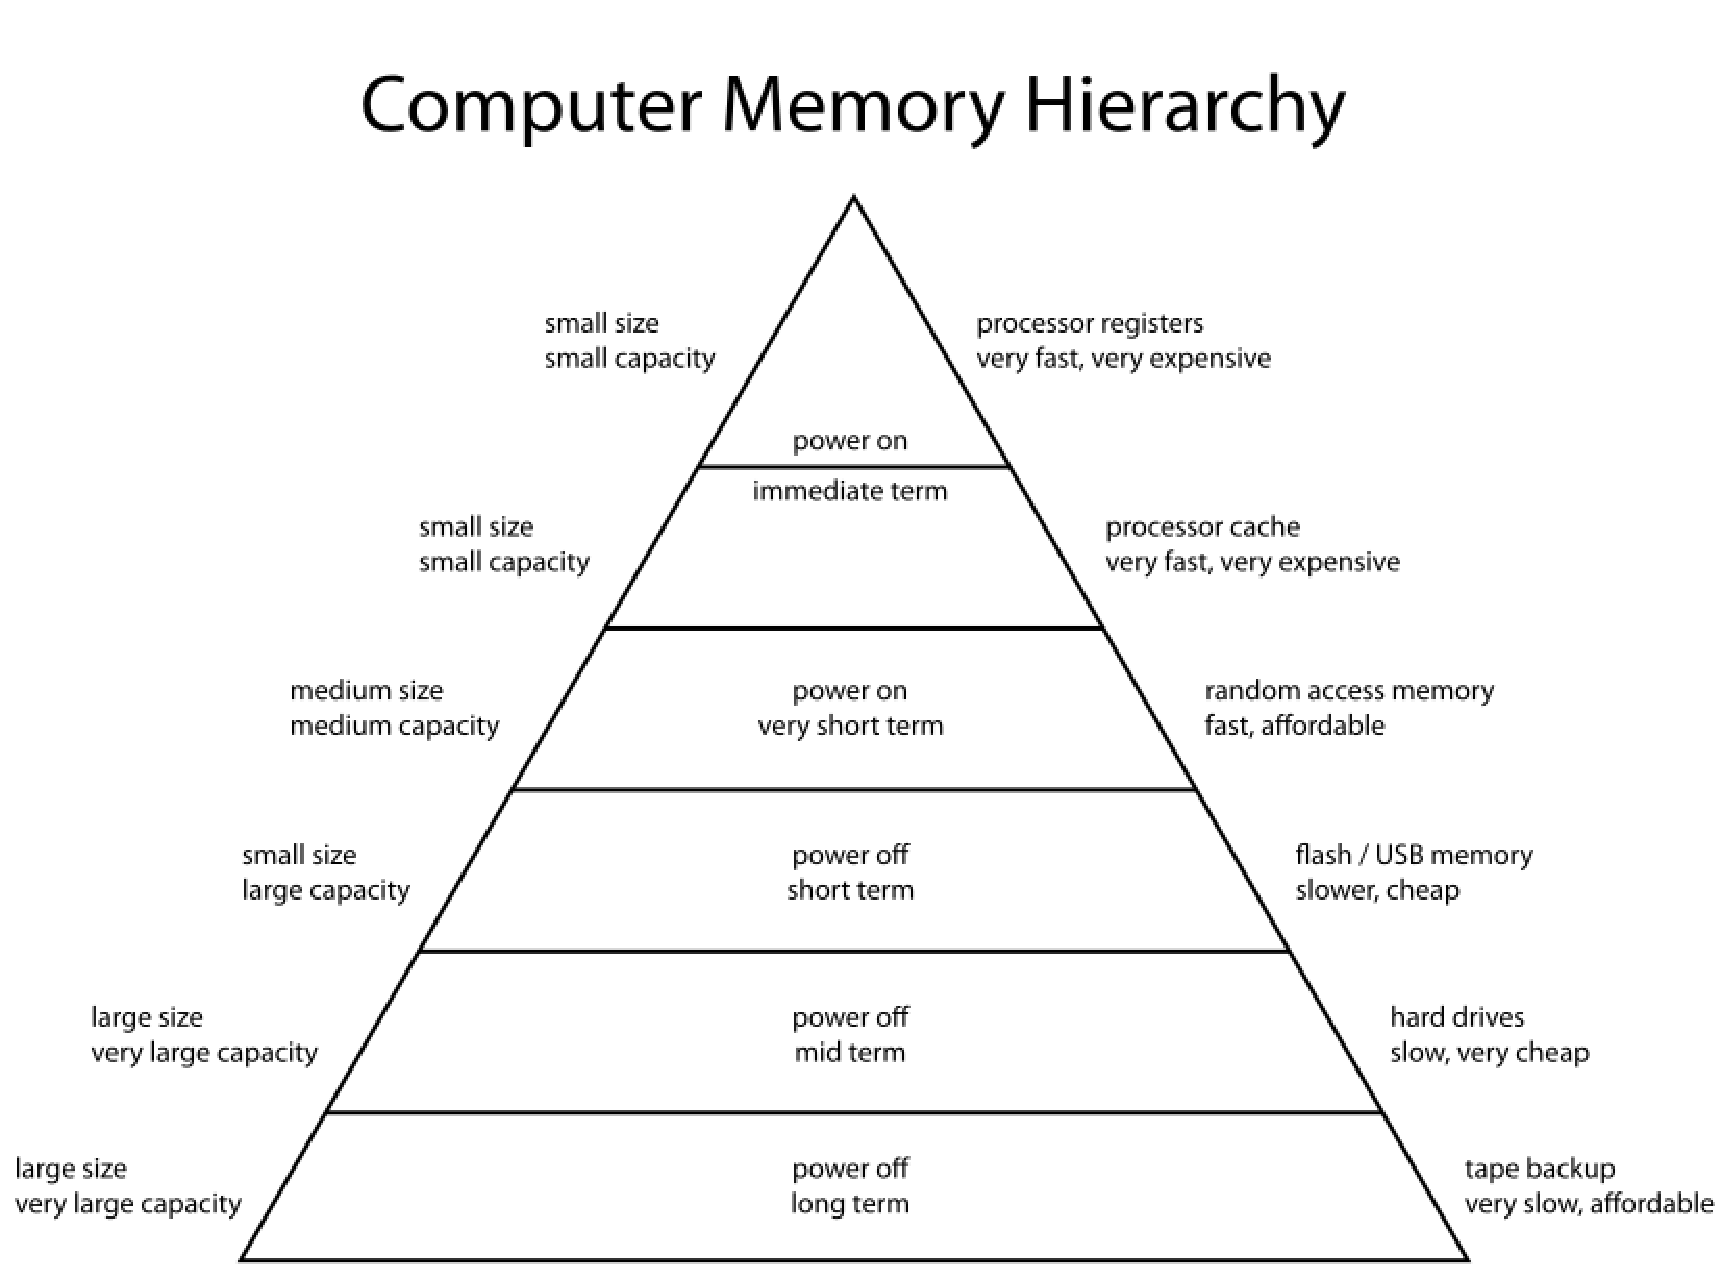
\includegraphics[width=0.8\textwidth]{images/mem-hier.pdf}}
	
	That's because every PC is built that way.

	\note[item]{Τρέχα}
\end{frame}

\begin{frame}
	Is there anything to help us?
	\dspc
	FACT: We are not the first to have speed issues\\
	Facebook, Twitter, Dropbox, every one has hit and surpassed their limits.
	\dspc
	There are solutions separated in two categories:
	\begin{itemize}
		\item Block-based caching
		\item Object-based caching
	\end{itemize}
	\note[item]{Τώρα που ξέρουμε τη λύση, υπάρχει κάτι που μπορούμε να 
		κάνουμε;}
	\note[item]{Υπάρχει κάτι έτοιμο; ΝΑΙ}
	\note[item]{Δυο κατηγορίες:
		\begin{itemize}
			\item βλέπουν τα δεδομένα σαν blocks ενός δίσκου
			\item βλέπουν τα δεδομένα σαν κομμάτια αντικειμένων
		\end{itemize}
		Διαφορά: \todo
	}
\end{frame}

\begin{frame}{Block-based caching solutions}

	Most notable examples:
	\begin{itemize}
		\item Bcache
		\item Flashcache
		\item EnhanceIO
	\end{itemize}
	\dspc
	Typically scale-up solutions.
	\dspc
	Pros: Simple, scale-up\\
	Cons: Unaware of CoW, kernel-space solutions, redundancy issues

	\note[item]{Δε θα επεκταθούμε γιατί έχουν κάποια βασικά κοινά:
		\begin{itemize}
			\item Kernel modules
			\item expose εικονικά block devices που δείχνουν σε 
				γρήγορα μέσα
			\item Καθαρά caching μηχανισμοί που παίζουν με writeback, 
				writethrough κτλ.
		\end{itemize}
	}
	\note[item]{Εξήγησε που μπαίνουν (xsegbd). ΠΗΓΑΙΝΕ στο archipelago}
	\note[item]{Παρότι είναι αρκετά απλοί, δε γνωρίζουν την CoW πολιτική 
		άρα χάνουν χώρο και είναι στον kernel (που δε θέλουμε)
	}
\end{frame}

\begin{frame}{Object-based caching solutions}
	Most notable examples:
	\begin{itemize}
		\item Memcached
		\item Couchbase
	\end{itemize}
	\dspc
	Typically scale-out solutions
	\dspc
	Pros: Distributed with no SPOF, can utilize unneeded RAM, user-space 
	solutions\\
	Cons: Memcached has no persistence, Couchbase cannot use RADOS as its 
	backend, more suitable for databases
	\note{Τα πράγματα γίνονται πιο ενδιαφέροντα εδώ:
		\begin{itemize}
			\item Κατανεμημένα συστήμα χωρίς ενιαίο σημείο 
				αποτυχίας (SPOF), μπορούν να τρέχουν εκτός host οπότε δεν το 
				επιβαρύνουν, είναι user-space λύσεις
			\item Memcached δε διατηρεί τα δεδομένα, couchbase δεν μπορεί να 
				μιλήσει με RADOS \end{itemize}
	}
\end{frame}

\begin{frame}{Conclusions}

	\begin{itemize}
		\item Most solutions far from Archipelago's logic
		\item Others not suited for storage and more suited for 
			databases
		\item Block-based caching might be good for the storage backend
		\item Must implement our own solution
	\end{itemize}

	\note{Οι λύσεις αυτές είναι μακριά από τη λογική και το I/O pipeline του 
		αρχιπελάγους. Είναι άσχετα συστήματα που πρέπει να επέμβουμε σε αυτά 
		για να κάνουμε αυτά που θέλουμε. Άρα πρέπει να κάνουμε τη δική μας 
		λύση}
\end{frame}
	
